%%%%%%%%%%%%%%%%%%%%%%%%%%%%%%%%%%%%%%%%%%%%%%%%%%%%%%%%%%%%%%%%%%%%%
%
% CSCI 1430 Written Question Template
%
% This is a LaTeX document. LaTeX is a markup language for producing documents. 
% You will fill out this document, compile it into a PDF document, then upload the PDF to Gradescope. 
%
% To compile into a PDF on department machines:
% > pdflatex thisfile.tex
%
% If you do not have LaTeX, your options are:
% - Personal laptops (all common OS): http://www.latex-project.org/get/ 
% + VSCode extension: https://marketplace.visualstudio.com/items?itemName=James-Yu.latex-workshop
% - Online Tool: https://www.overleaf.com/ - most LaTeX packages are pre-installed here (e.g., \usepackage{}).
%
% If you need help with LaTeX, please come to office hours.
% Or, there is plenty of help online:
% https://en.wikibooks.org/wiki/LaTeX
%
% Good luck!
% The CSCI1430 staff
%
%%%%%%%%%%%%%%%%%%%%%%%%%%%%%%%%%%%%%%%%%%%%%%%%%%%%%%%%%%%%%%%%%%%%%

\documentclass{csci1430}

\begin{document}
\title{Homework 4 Written Questions}
\maketitle
\thispagestyle{fancy}

\writeinstructions

\section*{This Homework}
\begin{itemize}
    \item 5 questions \textbf{[10 + 12 + 12 + 6 + 10 = 52 points]}.
    \item Include code, images, and equations where appropriate.
\end{itemize}


%%%%%%%%%%%%%%%%%%%%%%%%%%%%%%%%%%%%%%%%
\pagebreak
\begin{question}[points=10,drawbox=false]
\end{question}

\begin{subquestion}[points=2]
Define bias in machine learning and describe how to measure it. \textbf{[2--3 sentences.]}
\end{subquestion}

\begin{answer}[height=8]

\end{answer}
    
\begin{subquestion}[points=2]
Define variance in machine learning and describe how to measure it. \textbf{[2--3 sentences.]}
\end{subquestion}

\begin{answer}[height=8]

\end{answer}
    

\pagebreak
\begin{subquestion}[points=2]
Define overfitting in the context of evaluating a classifier and describe how to measure it.
\end{subquestion}
    
\begin{answer}[height=8]

\end{answer}
    

\begin{subquestion}[points=2]
Define underfitting in the context of evaluating a classifier and describe how to measure it.
\end{subquestion}
    
\begin{answer}[height=8]

\end{answer}
    

\begin{subquestion}[points=2]
How might we mitigate high bias?
How might we mitigate high variance?
\end{subquestion}
    
\begin{answer}[height=8]

\end{answer}


%%%%%%%%%%%%%%%%%%%%%%%%%%
\pagebreak
\begin{question}[points=12,drawbox=false] 
Suppose we are given a scene classification task and a dataset. Suppose also that we pick bag of words as the image representation for our classifier. `Bag of words' originated in text processing; for computer vision, a `word' is a visual feature.

The bag of words representation handles the spatial layout of information in a way that can be an advantage or a disadvantage in different cases.
\end{question}

\begin{subquestion}[points=2]
Describe two example scenarios when dealing with images: one that illustrates an advantage of the bag of words representation, and another that shows a disadvantage of the bag of words representation. \textbf{[5--6 sentences]}
\end{subquestion}

\begin{answer}[height=12]

\end{answer}


\begin{subquestion}[points=1]
Describe additional features or other information that you can add to your representation that might overcome the disadvantage of bag of words you stated above. \textbf{[2--4 sentences]}
\end{subquestion}

\begin{answer}[height=8]

\end{answer}


\pagebreak
Next, we define a feature transform for each image, and pick SIFT extracted in a sparse grid pattern. To reduce the size of our problem, we create a dictionary of visual words using k-means clustering upon all the features extracted from our images.

Examining the SIFT features generated from our training database tells us that many features are almost equidistant from two or more visual words.

\begin{subquestion}[points=1]
Why might this affect classification accuracy? \textbf{[2--4 sentences]}
\end{subquestion}
    
\begin{answer}[height=6]

\end{answer}
    

\begin{subquestion}[points=2]
Given the situation, describe \emph{two} methods to improve classification accuracy, and explain why they would help. (\emph{These can be for k-means, or otherwise.}) \textbf{[4--6 sentences]}
\end{subquestion}
    
\begin{answer}[height=12]

\end{answer}
    

\pagebreak
\begin{subquestion}[points=4]
How might we determine whether our classifier is a good model? Discuss technical solutions. \textbf{[5--6 sentences]}
\end{subquestion}

\begin{answer}[height=12]

\end{answer}

\begin{subquestion}[points=2]
After training, suppose we find that our model shows bad performance on our test data. When is it appropriate to pick a new test dataset for which our model achieves better performance? \textbf{[3--4 sentences]}
\end{subquestion}

\begin{answer}[height=12]

\end{answer}



\pagebreak
\begin{question}[points=12,drawbox=false]
The performance of a machine learning system is determined by the data we train it upon and the feature transforms and classifier optimizations we execute. Our perception of that performance is determined by how we evaluate and deploy machine learning systems. Performance limitations from the bias we discussed in Q1 is a \emph{learning bias}, and there are many other kinds of bias throughout the machine learning life cycle.

Another is \emph{evaluation bias}: that evaluation using overall accuracy can mask poor performance in specific subgroups.
Buolamwini and Gebru's 2018 paper \href{http://proceedings.mlr.press/v81/buolamwini18a/buolamwini18a.pdf}{Gender Shades: Intersectional Accuracy Disparities in Commercial Gender Classification} found that Microsoft's Face API trained gender classifier achieved 94\% overall accuracy, with 100\% accuracy on lighter-skinned male faces but only 79.2\% accuracy on darker-skinned female faces. In response to the report, Microsoft \href{https://blogs.microsoft.com/ai/gender-skin-tone-facial-recognition-improvement/}{significantly improved} their classifier's performance by making changes across their machine learning system. This occurred through ``expanded and revised training and benchmark datasets, new data collection efforts to further improve the training data by focusing specifically on skin tone, gender, and age, and an improved classifier to produce higher precision results.''

Suresh and Guttag describe \href{https://dl.acm.org/doi/10.1145/3465416.3483305}{seven kinds of bias in machine learning system life cycles}. To help you gain the language to talk about these issues, please read their article up to Section 4 (log-in through Brown to ACM Digital Library or PDF \href{https://drive.google.com/file/d/10YdCwZ0E0XBYS3oj_hfeI0TQ6lpepGKK/view}{here}) [15 minutes].

\vspace{3ex}
\hrule
\vspace{1ex}

In this homework, we will train a scene classifier using data from Lazebnik et al. 2006. Please review the data to check for potential biases: look at images in the data/train and data/test directories and consider their class labels. 

For example, if the street images in the dataset were used for training today, new buildings or the variation in the styles of cars and pedestrian clothings might bias the machine learning system. This could be a data \emph{historical bias} caused by out-of-date real-world sampling, among other potential biases. 
\end{question}

\pagebreak
\begin{subquestion}[points=4]
Please list at least two potential issues in the dataset and name their biases following Suresh and Guttag. There may be more than one bias per issue. \\

For each issue, please describe a potential consequence for an application that trained with this data. Is there one bias that seems to be more relevant to the dataset? \textbf{[2--3 sentences for each]}
\end{subquestion}

\begin{answer}[height=20]

\end{answer}

\pagebreak
Dataset curators might merge multiple sources to fill in gaps in sampling a data distribution. Upon limitations in Microsoft's Face API being revealed, its engineers were required to ``expand and revise training datasets''---perhaps in a hurry and under pressure. 

Please find additional scene data to add to the Lazebnik et al.~2006 dataset to reduce one of your issues. Here are two places to find datasets: \href{https://datasetsearch.research.google.com}{Google Dataset Search} and \href{https://www.kaggle.com}{Kaggle}, but you can propose to use any source you find.

\begin{subquestion}[points=4]
Find a dataset and provide a URL to it. Given one of your issues identified in Q3.1, describe how the new data addresses it. \\

How was this new data collected?
What values of the stakeholders that collected the data would be helpful to know in answering this question?
(Recall some of the values in our \href{https://browncsci1430.github.io/resources/ethics_primer/}{ethics resource}.)

\textbf{[4--5 sentences]}
\end{subquestion}

\begin{answer}[height=20]

\end{answer}

\pagebreak
Microsoft's engineers also conducted ``new data collection efforts.'' With many potential pitfalls, data collection can be a daunting task.
One approach that researchers and companies have used to ease cost and time investment is 
\href{https://en.wikipedia.org/wiki/Web_scraping#}{web scraping}, which downloads data across many websites to more easily create large datasets. 

Web scraping has come under increased scrutiny as computer vision systems have been deployed in real-world applications, because the technical capability to download publicly-accessible data does not imply consent for the use of that data. In 2021, France found that Clearview AI, a company that operates a facial recognition platform for law enforcement, violated privacy laws by scraping 10 billion images of people's faces from Facebook, YouTube, and other websites without consent; Clearview AI was fined \href{https://www.edpb.europa.eu/news/national-news/2022/french-sa-fines-clearview-ai-eur-20-million\_en}{€20 million} under the EU's General Data Protection Regulation (GDPR) law.


\begin{subquestion}[points=4]
The Lazebnik et al.~15-scene dataset was collected using a combination of personal images, licensed photo collections, and web scraping. \\
    
Suppose you were a machine learning engineer tasked with collecting \emph{new} scene data yourself. You are not given clear specifications as to how you should collect the images. Name three stakeholders you would engage to increase your success and explain why. \textbf{[6--8 sentences]}
\end{subquestion}

\begin{answer}[height=20]

\end{answer}

%%%%%%%%%%%%%%%%%%%%%%%%%%%%%%%%%%%%5
\pagebreak
\begin{question}[points=6]
\textbf{Code preparation.}\\
Given a linear classifier such as SVM which separates two classes (binary decision), we wish to use multiple linear classifiers to separates $k$ classes. \\

On the next page, we provide pseudo-code for a linear classifier. It fits the classifier to a training set, and then classifies a new test example into one of two classes. Please edit the pseudo-code to convert this into a multi-class classifier. 
\end{question}

\emph{Note:} A more efficient software application would separate the classifier training and testing into two different functions so that the model could be reused without retraining. Feel free to ignore this for now.

\vspace{2ex}
\hrule
\vspace{1ex}

You can take either the one vs.~all approach (also called the one vs.~many or one vs.~others) or the one vs.~one approach; please declare which approach you take.

Select the implementation you chose:

\begin{answerlist}
    \item One vs.~all % Use \item[\done]
    \item One vs.~one
\end{answerlist}

\emph{Be aware that:}
\begin{enumerate}
    \item The input labels in the multi-class case are different, and you will need to match the expected label input for the \texttt{train\_linear\_classifier} function.
    \item You need to make a new decision on how to aggregate or decide on the most confident prediction.
\end{enumerate}


\pagebreak
\begin{answer}[height=30]
\begin{python}
# Inputs and Outputs for binary classifier
# Inputs:
# - train_feats: N x d matrix of N features each d dims. long
# - train_labels: N x 1 array of -1 (class 0) or 1 (class 1)
# - test_feat: 1 x d image for which we wish to predict a label
#
# Outputs: -1 (class 0) or 1 (class 1)
#
# Inputs and Outputs for multi-class classifier from 0 to k-1
# Inputs: As before, except
# - train_labels: N x 1 array of class integers from 0 to k-1
# 
# Outputs: A class label integer from 0 to k-1

# TODO: Turn this into a multi-class classifier for k classes.
def classify(train_feats, train_labels, test_feat)
    # Train classification hyperplane
    weights, bias = train_linear_classifier(train_feats, train_label)
    # Compute distance from hyperplane
    test_score = weights * test_feats + bias

    return 1 if test_score > 0 else -1
    
\end{python}
\end{answer}


\pagebreak
\begin{answer}[height=40]
\begin{python}
# Extra page if you need it            
\end{python}
\end{answer}



%%%%%%%%%%%%%%%%%%%%%%%%%%%%%%%%%%%%%%%%%%
\pagebreak
\begin{question}[points=10,drawbox=false] 
\textbf{Code preparation.}\\
We will use a feature transform called HOG---`Histogram of Oriented Gradients'. As its name implies, it works similarly to SIFT. In classification, we might extract many HOG features across the entire image (not just at corners) to create visual words.

HOG creates one feature descriptor per image `block'. Each block is split into `cells' covering pixels. HOG outputs a 9-bin histogram of oriented gradients per cell. We append these together to obtain the feature descriptor for each block. As a result, if we have $(z,z)$ cells per block, the feature descriptor for each block will be of size $z \times z \times 9$. In other words, computing HOG over the whole image produces a matrix where each row is a descriptor. 

\emph{Blocks can overlap as displayed in the diagram below.}

\begin{center}
    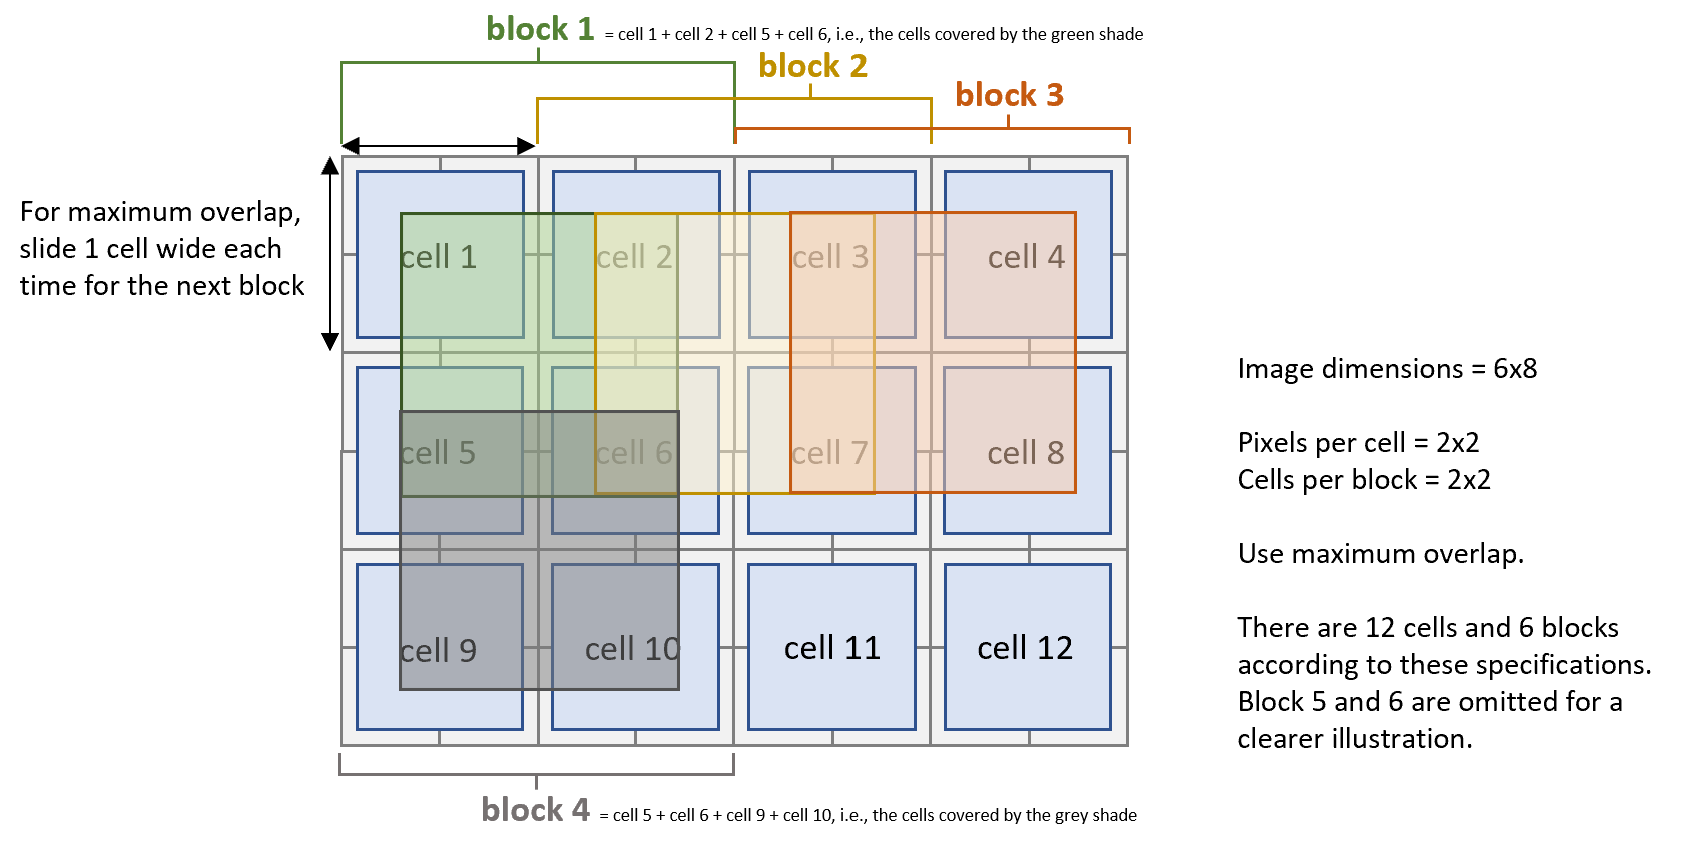
\includegraphics[width=\linewidth]{images/hog-diagram.png}
\end{center}
\end{question}


\pagebreak
Given a $72\times72$ image, calculate the number of cells, blocks, and feature descriptor size that will occur when we extract one HOG feature with the following parameters using maximum overlap between blocks.

\begin{subquestion}[points=3]
Scenario 1: Pixels per cell = $4\times4$, cells per block = $4\times4$ \end{subquestion}

\begin{answer}
Number of cells:
\end{answer} 

\begin{answer}
Number of blocks:
\end{answer} 
    
\begin{answer}[height=3]
Dimensions of resulting single feature descriptor for the whole image:
\end{answer} 


\begin{subquestion}[points=3]
Scenario 2: Pixels per cell = $8\times8$, cells per block = $2\times2$.
\end{subquestion}

\begin{answer}
Number of cells:
\end{answer} 

\begin{answer}
Number of blocks:
\end{answer} 
    
\begin{answer}[height=3]
Dimensions of resulting single feature descriptor for the whole image:
\end{answer}


\pagebreak
\begin{subquestion}[points=4]
When using HOG, the parameters such as pixels per cell and cells per block impact the resulting feature descriptor and so our performance on a classification task. \\

What are the pros and cons of the two parameter combinations? Which might you expect to have better performance, and why? \textbf{[3--6 sentences]}
\end{subquestion}

\begin{answer}[height=10]

\end{answer}


%%%%%%%%%%%%%%%%%%%%%%%%%%%%%%%%%%%
% \emph{Note: You may find it interesting to read the thesis of Navneet Dalal (co-inventor of HOG) for more information on this topic. \href{http://lear.inrialpes.fr/people/dalal/NavneetDalalThesis.pdf}{[Link to thesis]} (pages 39, 41 in Section 4.3).}
%%%%%%%%%%%%%%%%%%%%%%%%%%%%%%%%%%%


\pagebreak
\section*{Feedback? (Optional)}
We appreciate your feedback on how to improve the course. You can provide anonymous feedback through \href{https://forms.gle/Eu5jJbDUmLknAyJV9}{this form} which can be accessed using your Brown account (your identity will not be collected). If you have urgent non-anonymous comments/questions, please email the instructor.


% \pagebreak
% \section*{Students: Any additional pages would go here.}


\end{document}